\documentclass[french]{beamer}
\usefonttheme[onlymath]{serif}

\usepackage[utf8]{inputenc}
\usepackage[T1]{fontenc}
\usepackage{lmodern}
\usepackage{babel}
\usepackage{tikz}
\usepackage{smartdiagram}
\usepackage[babel]{csquotes}
\usepackage[url=false, doi=false, style=science, backend=bibtex, bibencoding=ascii]{biblatex}
%\bibliography{IEEEabrv,bib/OAM}


\graphicspath{{img/}{../}}

\usepackage{../beamerthemeulaval}
\usepackage{../beamercolorthemeulaval}
\logo{\includegraphics[height=0.5cm]{UL_P}\hspace{.2cm}\vspace{.85\paperheight}}
\newcommand\red[1]{{\color{ulred}{\textbf{#1}}}}

\mode<presentation> {
	\setbeamercovered{invisible}
	\setbeamertemplate{navigation symbols}{} % Enlever les icônes de navigation
}




\title[Méthode Scientique]{La méthode scientifique en génie et en apprentissage automatique}
%\subtitle[]{}

\author[C. Besse]{Camille Besse}
\institute[Université Laval]
{
	Départment d'Informatique et de Génie Logiciel\\
	Université Laval, Québec, Canada \\
	\medskip
	{\emph{camille.besse@ift.ulaval.ca}}
}
%\date{\today} % \today will show current date. 
% Alternatively, you can specify a date.


\AtBeginSection[]{
  \begin{frame}
	\Huge \centerline{\insertsection}
%  \small \tableofcontents[currentsection, hideothersubsections]
  \end{frame} 
}

\begin{document}



%---------------------------------------------------------------------------------------------------------------------------------------- 
\begin{frame}[label=titre, plain]
	\titlepage
	\begin{center}\includegraphics[height=1cm]{UL_P}\end{center}
	
	{\tiny Sources : \\ 
		Marzuki B. Khalid : Research Methodology\\ Christine Dufour :  \href{http://reseauconceptuel.umontreal.ca/rid=1QVBNNBB9-1B7N610-4SQ/sci6060_c01_rexploratoire_rdescriptive_rexplicative.cmap}{Recherche et méthode scientifique}}
\end{frame}


\section*{Contents}

%---------------------------------------------------------------------------------------------------------------------------------------- 
\begin{frame}[label=toc]{Outline}
	\setlength{\leftskip}{5cm}%
	\tableofcontents[subsectionstyle=show]
\end{frame}

\section{La recherche, c'est quoi ?}

%---------------------------------------------------------------------------------------------------------------------------------------- 
\begin{frame}{Exemples}
\begin{itemize}
	\item<1-> Toto a écrit un rapport sur l’usage d’internet au Québec, après avoir bien étudié la littérature sur le sujet \\ Est ce de la recherche ? \uncover<2->{\red{non}}
	\item<3-> Mario a complété une recherche sur le personnel de la FSG et complété un document qui donne des infos sur l’âge, le salaire, les liens sociaux, etc. \\ Est ce de la recherche ? \uncover<4->{\red{non}}
	\item<5-> Jules a participé à un atelier pour le développement et préparé un rapport technique donnant quelques "recettes". Il a fait pour cela une revue de la littérature et a questionné les intervenants du workshop. \\ Est ce de la recherche ? \uncover<6->{\red{non}}
\end{itemize}
\end{frame}


%---------------------------------------------------------------------------------------------------------------------------------------- 
\begin{frame}{Exemples suite}
Seb gestionnaire d’une compagnie assemblant des PCs, reçoit des plaintes d’utilisateurs : après quelques mois, la carte mère est HS.
	\begin{itemize}
		\item Seb demande aux techniciens les informations nécessaires en vue d’identifier les facteurs qui ont influencé le problème;
		\item Seb identifie plusieurs problèmes potentiels et émet des hypothèses; 
		\item Seb construit une grille de tests et demande à des utilisateurs les informations nécessaires pour la remplir;
		\item Seb analyse les données obtenues de la part des utilisateurs, interprète les résultats à la lumière des hypothèses et tire ses conclusions.
	\end{itemize}
Est ce de la recherche ? \uncover<2->{\red{oui !}}
\end{frame}

%---------------------------------------------------------------------------------------------------------------------------------------- 
\begin{frame}{Qu’est ce que la recherche ?}
Dans l’exemple précédent :
	\begin{itemize}
		\item Seb, y va à travers une séquence d’étapes ordonnées et donc systématiques;
		\item Seb, ne saute pas directement aux conclusions, mais utilise une \red{méthode} scientifique qui consiste à investiguer en vue d’atteindre des	conclusions;
		\item Deux caractéristiques importantes de la recherche : Généralement une \red{procédure systématique} qui suit une \red{méthode scientifique}	d’investigation.
	\end{itemize}
\end{frame}

%---------------------------------------------------------------------------------------------------------------------------------------- 
\begin{frame}{Tentative de définition}
La recherche est : 
	\begin{itemize}
		\item la poursuite de faits ou de vérités sur un sujet
		\item  une investigation organisée méthodologiquement
		\begin{itemize}
			\item voulant résoudre des problèmes,
			\item en testant des hypothèses,
			\item pour finalement inventer de nouveaux produits.
		\end{itemize}
	\end{itemize}
\end{frame}

%---------------------------------------------------------------------------------------------------------------------------------------- 
\begin{frame}{Tentative de définition}
La recherche est systématique dans la mesure où elle suit des étapes ordonnées de manière logique :
	\begin{itemize}
		\item Comprendre la nature du problème étudié et identifier les champs de connaissances qui y sont liés;
		\item Établir l’état de l’art, i.e. collecter/étudier la littérature pour comprendre le problème a déjà été approché;
		\item Collecter les données de manière organisée et contrôlée en vue d’arriver à des décisions valides;
		\item Analyser les données appropriées au problème étudié;
		\item Tirer les conclusions qui s’imposent et faire les généralisations qu’il faut.
	\end{itemize}
\end{frame}

%---------------------------------------------------------------------------------------------------------------------------------------- 
\begin{frame}{Schéma idéal de recherche}
\begin{center}
\resizebox{!}{0.8\textheight}{
	\begin{tikzpicture}
		\filldraw[fill=ulred] (0,8)rectangle +(10,1) node[pos=.5, text=white,font=\bfseries,minimum height=1cm](P) {Identifier et formuler le problème};
		\filldraw[fill=ulred] (0,6)rectangle +(10,1) node[pos=.5, text=white,font=\bfseries,minimum height=1cm](E) {État de l'art};
		\filldraw[fill=ulred] (0,4)rectangle +(10,1) node[pos=.5, text=white,font=\bfseries,minimum height=1cm](C) {Collecte des données};
		\filldraw[fill=ulred] (0,2)rectangle +(10,1) node[pos=.5, text=white,font=\bfseries,minimum height=1cm](A) {Analyse des données, traitement et résultats};
		\filldraw[fill=ulred] (0,0)rectangle +(10,1) node[pos=.5, text=white,font=\bfseries,minimum height=1cm](T) {Tirer les conclusions et généralisations};
		\draw[-latex, ultra thick, ulred] (P.south) -- (E.north);
		\draw[-latex, ultra thick, ulred] (E.south) -- (C.north);
		\draw[-latex, ultra thick, ulred] (C.south) -- (A.north);
		\draw[-latex, ultra thick, ulred] (A.south) -- (T.north);
	\end{tikzpicture}}
\end{center}
\end{frame}

%---------------------------------------------------------------------------------------------------------------------------------------- 
\begin{frame}{Les propriétés souhaitées de la recherche}
\begin{itemize}
	\item Elle est reproductible;
	\item Elle est incrémentale car souvent basée sur le travail d’autrui;
	\item Elle est généralisable et transférable à d’autres contextes;
	\item Elle est basée sur des arguments logiques et attachée à une théorie;
	\item Elle soulève de nouvelles questions;
	\item Elle est apolitique, éthique, objective,...  
\end{itemize}
\end{frame}

%---------------------------------------------------------------------------------------------------------------------------------------- 
\begin{frame}{Les propriétés NON souhaitées de la recherche}
\begin{itemize}
	\item Tout l'opposé
	\item S'acharner à vouloir montrer quelque chose qui n'existe pas;
	\item Copier le travail d'autrui;
	\item Falsifier des données pour montrer quelque chose;
	\item Masquer ou déformer de l'information disponible dans le but de tromper.
\end{itemize}
\end{frame}

%---------------------------------------------------------------------------------------------------------------------------------------- 
\begin{frame}{C'est quoi faire de la recherche ?}
\begin{itemize}
	\item Faire de la recherche, c'est suivre une méthode scientifique
	\item I.e. faire un usage intégré de raisonnements \red{déductifs} et \red{inductifs}
	\item Cela permet d'expliquer et/ou prédire certains phénomènes
	\item Un postulat de base de la méthode scientifique est que \red{tout phénomène a une cause}.
\end{itemize}
\end{frame}

%---------------------------------------------------------------------------------------------------------------------------------------- 
\begin{frame}{C'est quoi faire de la recherche ?}
\begin{itemize}
	\item Cela commence par la construction d'hypothèses depuis des observations ponctuelles et une connaissance du domaine (induction)
	\item vers la construction d'hypothèses sur les conséquences ou implications possibles (déduction)
	\item suivi par le tests de ces implications pour la comfirmation ou la rejection des hypothèses.
	\item[$\Rightarrow$] L'usage intégré de l'induction et de la déduction est l'essence de la méthode scientifique.
\end{itemize}
\end{frame}

%---------------------------------------------------------------------------------------------------------------------------------------- 
\begin{frame}{}
\begin{center}
	\tikzset{every shadow/.style={fill=none,shadow scale=0}}
	\smartdiagramset{
	uniform color list=white for 8 items,
	border color=none,
	module minimum width=3cm, 
	module shape=rectangle,
	text width=3cm,
	circular distance=3.5cm,
	}
	\smartdiagram[circular diagram:clockwise]{Produire de nouvelles questions,Poser une question, Indentifier les facteurs, Formuler des hypothèses, Collecter des données, Tester les hypothèses, Suivre les implications des hypothèses, Reconsidérer la théorie}
	
	\vspace{-0.69\textheight}
	\smartdiagramset{
	uniform color list=white for 4 items,
	border color=none,
	module minimum width=0cm, 
	module shape=circle,
	text width=0cm,
	circular distance=2cm,
	uniform arrow color=true,
	arrow color=ulred
	}
	\smartdiagram[circular diagram:clockwise]{,,,}
	
\end{center}
\end{frame}

\section{Classifier la recherche}

%---------------------------------------------------------------------------------------------------------------------------------------- 
\begin{frame}{Les types de recherche}
\begin{itemize}
	\item Passer en revue les recherches passée est une étape importante de la recherche
	\item Cela aide à la formulation du problème, à la constrution d'hypothèse, et à la sélection de schémas comparatifs
	\item Il vous faut donc positionner votre recherche dans une certaine catégorie
	\item Chaque catégorie utilise un ensemble spécifique de procédures
\end{itemize}
\end{frame}

%---------------------------------------------------------------------------------------------------------------------------------------- 
\begin{frame}{}
\begin{center}
	\begin{huge}
		On a trois grands types:
		
		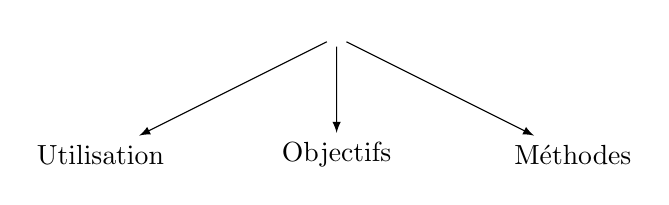
\begin{tikzpicture}[sibling distance=3cm,-latex]
		\node{}
			child {node {Utilisation}}
			child {node {Objectifs}}
			child {node {Méthodes}};
		\end{tikzpicture}
	\end{huge}
\end{center}
\end{frame}

\subsection{Selon l'utilisation}

%---------------------------------------------------------------------------------------------------------------------------------------- 
\begin{frame}{La recherche selon son utilisation}
\begin{center}
		Exprime le degré avec lequel les résultats de recherche sont applicables et généralisables à l'enseignement et à la vie pratique.
		
		\vspace{1cm}
	\begin{huge}		
		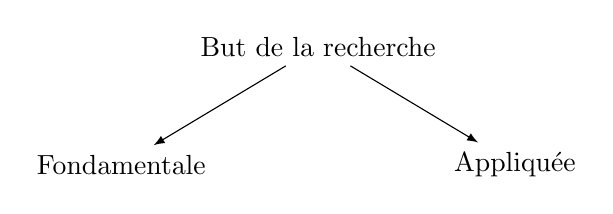
\begin{tikzpicture}[sibling distance=5cm,-latex]
		\node{But de la recherche}
		child {node {Fondamentale}}
		child {node {Appliquée}};
		\end{tikzpicture}
	\end{huge}
\end{center}
\end{frame}

%---------------------------------------------------------------------------------------------------------------------------------------- 
\begin{frame}{La recherche fondamentale et appliquée}
\begin{itemize}
	\item Fondamentale : qui vise à éprouver des théories, des lois, des principes. afin d'accroître les connaissances dans un domaine et ce, sans préoccupation pratique immédiate
	\item Appliquée : qui ivse à trouver des solutions pratiques à des problèmes pratiques
\end{itemize}
Mais à quoi ca sert ? [critiques usuelles]: 
\begin{itemize}
	\item Fondamentale : Perte d'argent et de temps puisqu'il n'y a pas d'application "réelle" ... \emph{pelletage de nuage} ... 
	\item Appliquée : Pas serieux, non généralisable (rapide et petite-échelle), utile à court terme seulement ...
\end{itemize}
Oui ... mais les deux types de recherche se nourrissent l'une de l'autre.
\end{frame}

%---------------------------------------------------------------------------------------------------------------------------------------- 
\usetikzlibrary{calc,trees,positioning,arrows,%
decorations.pathreplacing,decorations.pathmorphing,%
matrix}

\begin{frame}{La recherche fondamentale et appliquée}
\begin{center}
\tikzset{
	>=stealth',
	entity/.style={
		rectangle, 
		rounded corners, 
		top color=ulred, bottom color=white,drop shadow,
		text=black, very thick,
		text width=10em, 
		minimum height=3em, 
		text centered},
	line/.style={draw=ulred,ultra thick,-latex,shorten >=5pt,shorten <=5pt},
}
\resizebox{\textwidth}{!}{
	\begin{tikzpicture}
	\node[entity] (the) {Théorie/Loi};
	\node[entity] (hyp) [below right=2.28cm] {Hypothèses};
	\node[entity] (obs) [below=4cm] {Observations} ;
	\node[entity] (gen) [below left=2.28cm] {Généralisations empiriques} ;
	\draw[line] (the.east) to[bend left] node[midway, above right]{découlent} (hyp.north) ;
	\draw[line] (hyp.south) to[bend left] node[midway, below right,,text width=2.5cm,text centered]{se vérifient par} (obs.east);
	\draw[line] (obs.west) to[bend left] node[midway, below left,text width=2.5cm,text centered]{produisent par induction} (gen.south);
	\draw[line] (gen.north) to[bend left] node[midway, above left]{produisent} (the.west);
	
	\draw[decorate, decoration={brace},line width=1pt] let \p1=(the.north), \p2=(hyp.south), \p3=(hyp.east) in
	([xshift=2pt]$(\x3, \y1)$) -- ([xshift=2pt]$(\x3, \y2)$) node[midway, right=2pt] {Fondamentale};
	\draw[decorate, decoration={brace},line width=1pt] let \p1=(gen.north), \p2=(obs.south), \p3=(hyp.east) in
	([xshift=5pt]$(\x3, \y1)$) -- ([xshift=5pt]$(\x3, \y2)$) node[midway, right=2pt] {Appliquée};
	\end{tikzpicture}}
\end{center}
\end{frame}

\subsection{Selon les objectifs}
%---------------------------------------------------------------------------------------------------------------------------------------- 
\begin{frame}{La recherche par objectif poursuivi}
En fonction de la natude des questions posées
\begin{center}
		\resizebox{\textwidth}{!}{
			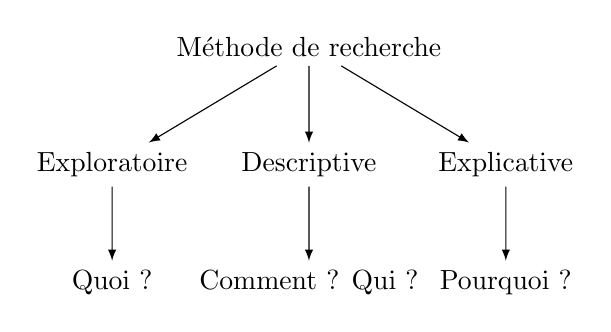
\begin{tikzpicture}[sibling distance=2.5cm,-latex]
			\node{Méthode de recherche}
			child {node {Exploratoire} 
				child {node {Quoi ?}}}
			child {node {Descriptive} 
				child {node {Comment ? Qui ?}}}
			child {node {Explicative} 
				child {node {Pourquoi ?}}};
			\end{tikzpicture}}
\end{center}
\end{frame}

\subsubsection{Recherche exploratoire}

%---------------------------------------------------------------------------------------------------------------------------------------- 
\begin{frame}{La recherche exploratoire : QUOI ?}
Pour des phénomènes nouveaux, peu ou pas documentés.
\begin{itemize}
	\item Se familiariser avec des faits, des données, des situations et des questions de base
	\item Formuler des questions pour des recherches futures
	\item Générer de nouvelles idées, conjectures ou hypothèses
\end{itemize}
\end{frame}


\subsubsection{Recherche descriptive}

%---------------------------------------------------------------------------------------------------------------------------------------- 
\begin{frame}{La recherche descriptive : COMMENT ? QUI ?}
Pour des phénomènes que l'on connaît un peu et que l'on veut décrire en profondeur
\begin{itemize}
	\item Fournir une image détaillée et très précise
	\item Trouver de nouvelles données qui appuient ou contredisent d'anciennes données
	\item Clarifier une série d'étapes (processus)
	\item Documenter un processus ou mécanisme causal
\end{itemize}
La frontière entre recherche exploratoire et descriptive est parfois floue. Dans la pratique, on parle de recherche exploratoire-descriptive.
\end{frame}

\subsubsection{Recherche explicative}

%---------------------------------------------------------------------------------------------------------------------------------------- 
\begin{frame}{La recherche explicative : POURQUOI ?}
Pour des phénomènes connus, déjà décrits, pour lesquels on veut comprendre pourquoi les choses sont comme elles sont
\begin{itemize}
	\item Tester un théorie
	\item Élaborer et enrichir l'explication d'une théorie
	\item Supporter ou réfuter un explication
	\item Déterminer quelle explication parmi plusieurs est la meilleure
\end{itemize}
\end{frame}


\subsection{Selon les méthodes}

%---------------------------------------------------------------------------------------------------------------------------------------- 
\begin{frame}{La recherche par méthode employée}
En fonction des fondements philosophiques qui diffèrent selon les perceptions individuelles de la réalité, de la science, et de la nature humaine.
\begin{center}
	\resizebox{\textwidth}{!}{
		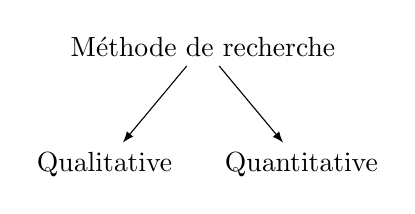
\begin{tikzpicture}[sibling distance=2.5cm,-latex]
		\node{Méthode de recherche}
		child {node {Qualitative}}
		child {node {Quantitative}};
		\end{tikzpicture}}
\end{center}
\end{frame}

\subsubsection{Méthode qualitative}

%---------------------------------------------------------------------------------------------------------------------------------------- 
\begin{frame}{La recherche par méthode qualitative : naturaliste}

Pour comprendre un phénomène selon la perspective des sujets, en contexte.
\begin{itemize}
	\item La réalité est multiple et se découvre dynamiquement en interagissant avec l'environnement : Connaissance relative ou contextuelle
	\item Les phénomènes humains sont uniques et non prévisibles
\end{itemize}
Critiques venant des "quantitatifs":
\begin{itemize}
	\item Manque de fiabilité, mensonges et biais humains dans les réponses au entrevues
	\item Biais inconscients dans l'analyse des résultats par les croyances des chercheurs
\end{itemize}
\end{frame}

%---------------------------------------------------------------------------------------------------------------------------------------- 
\begin{frame}{La recherche par méthode quantitative : positiviste logique}

Pour décrire, vérifier des relations entre des variables, et examiner les changements observés chez la variable dépendante, à la suite de la manipulation de la variable indépendante.
\begin{itemize}
	\item La réalité est percue comme unique et statique mais probabiliste.
	\item Les phénomènes humains sont prévisibles et contrôlables
	\item Les faits objectifs existent en dehors du chercheur et peuvent être découverts : connaissance absolue
\end{itemize}
Critiques venant des "qualitatifs":
\begin{itemize}
	\item Manque de pertinence : on cherche à tout mesurer avec parfois des variables inadéquates
	\item Il est possible de faire dire n'importe quoi à des chiffres si l'on ne fait pas attention
\end{itemize}
\end{frame}


\section{Le processus de la recherche}
%---------------------------------------------------------------------------------------------------------------------------------------- 
\begin{frame}{La recherche scientifique : un processus systématique}
\begin{center}
	\smartdiagramset{
	uniform color list=ulred for 6 items,
	border color=none,
	module minimum width=3cm, 
	module shape=rectangle,
	text width=3cm,
	circular distance=3.5cm,
}
\resizebox{!}{0.8\textheight}{
\smartdiagram[descriptive diagram]{
	{Problème,{Identifier/formuler le problème de manière claire et concise}},
	{Littérature, {Ressortir l'existant de l'état de l'art pour en identifier les lacunes}},
	{Méthode, {Choix de la méthodologie et des mesures de performance}},
	{Données, {Colligation/traitement des données}},
	{Analyse, {Analyse des données et production des modèles}},
	{Résultats, {Formulation des résultats et présentation}},
}}
\end{center}
\end{frame}

\subsection{Problème}
%---------------------------------------------------------------------------------------------------------------------------------------- 
\begin{frame}{Identifier le problème}
Ceci est le point de départ de toute recherche : c’est l’aspect le plus ardu de la recherche. Un problème \red{sous ou sur spécifié} risque d’engendrer pas mal de difficultés par la suite.
\begin{itemize}
	\item Spécifier le problème précisément;
	\item Identifier les variables et les définir adéquatement;
	\item Générer des hypothèses ou donner explicitement les questions de recherche;
	\item Évaluer le problème quant à son importance d’un point de vue recherche;
	\item Lier le problème posé à \red{l’état de l’art} et voir comment il a été approché et quelles méthodes ont été utilisées.
\end{itemize}
\end{frame}

%---------------------------------------------------------------------------------------------------------------------------------------- 
\begin{frame}{Identifier le problème : en AA}
\begin{itemize}
	\item Définir le problème à résoudre selon le domaine d'application, les contraintes et le contexte d'utilisation de la solution
	\item Identifier les variables d'entrées et de sorties, et les définir adéquatement, elles seront révisées au besoin si des variables exogènes ont a être ajoutées
	\item Générer des hypothèses sur les structures possibles de la résolution à valider
	\item Évaluer le problème quant à son importance du point de vue du résultat de l'application de la solution
	\item Lier le problème posé à \red{l’état de l’art} et voir comment il a été approché et quelles méthodes ont été utilisées dans des applications similaires
\end{itemize}
\end{frame}

\subsubsection{État de l'art}
%---------------------------------------------------------------------------------------------------------------------------------------- 
\begin{frame}{L'état de l'art : Revue de littérature}
C'est quoi ? 
\begin{itemize}
	\item Lire les précédents travaux sur le sujet
	\item Assurer le caractère incrémental de la recherche 
	\item Assurer la pertinence de la recherche
\end{itemize}
Objectifs : 
\begin{itemize}
	\item Circonscrire et préciser le problème
	\item Trouver de appoches existantes pour comparaison
	\item Éviter des répétitions ou des approches inefficaces
\end{itemize}
\end{frame}

%---------------------------------------------------------------------------------------------------------------------------------------- 
\begin{frame}{Revue de littérature : Comment Google Scholar}
Plusieurs techniques possibles : 
\begin{itemize}
	\item Définir les termes de la recherche
	\item Effectuer plusieurs recherches à l'aide de synonymes si possible
	\item Trouver un arcicle effectuant la revue de littérature sur le problème si possible
	\item Sinon, trouver au moins un article décrivant et résolvant le problème considéré
	\item Une fois une référence pertinente trouvée, chercher parmi les articles le citant, et parmi ceux cités par lui
\end{itemize}
\end{frame}

%---------------------------------------------------------------------------------------------------------------------------------------- 
\begin{frame}{Revue de littérature : Comment lire un article}
Mon algorithme personnel  pour accélerer la lecture, si un point semble pertinent passer au suivant, sinon, changer d'article
\begin{enumerate}
	\item Résumé : pour cerner le contenu
	\item Conclusion : pour valider rapidement les résultats obtenus
	\item Introduction : pour assurer que le problème est bien le même
	\item Revue de littérature : pour ajouter les articles pertinents dans le pipeline de lecture
	\item Résultats : pour comprendre les résultats obtenus
	\item Méthodologie : pour valider qu'elle est adéquate et pertinente
\end{enumerate}
Si vous vous êtes rendus à la méthodologie, une relecture complète et en profondeur de l'article est de mise dans le futur.
\end{frame}

\subsection{Méthodologie}
%---------------------------------------------------------------------------------------------------------------------------------------- 
\begin{frame}{Décrire la méthodologie}
Une fois le problème bien posé; il convient
	\begin{itemize}
		\item d’identifier le type de méthode de recherche et les méthodes elles-même; 
		\item de spécifier les sujets à étudier (les objets d’étude);
		\item de sélectionner adéquatement les échantillons, les données, etc.
		\item de sélectionner/construire des méthodes fiables pour faire les mesures des variables;
		\item d'établir et décrire le protocole de recherche en étapes claires.
	\end{itemize}
\end{frame}

%---------------------------------------------------------------------------------------------------------------------------------------- 
\begin{frame}{Décrire la méthodologie : en AA}
\begin{itemize}
	\item d’identifier le type de méthode à employer, généralement  quantitative, mais pourrait être exploratorie/descriptive;
	\item d'identifier les techniques qui vont être employées pour faire les modèles;
	\item de spécifier les objets à étudier qui ont été décomposés en caractéristiques;
	\item de construire une méthode fiable pour faire la colligation et le prétraitement des données;
	\item d'établir et décrire le protocole de recherche en étapes claires et reproductibles.
\end{itemize}
\end{frame}

\subsection{Données}
%---------------------------------------------------------------------------------------------------------------------------------------- 
\begin{frame}{Colliger/traiter les données}
	\begin{itemize}
		\item Manipuler adéquatement les variables expérimentales;
		\item Utiliser l’instrumentation pour mesurer les variables;
		\item Observer et collecter les informations nécessaires;
		\item Préparer les données en vue de l’analyse et de la modélisation;
		\item Documenter la préparation.
	\end{itemize}
\end{frame}

%---------------------------------------------------------------------------------------------------------------------------------------- 
\begin{frame}{Colliger/traiter les données : en AA}
\begin{itemize}
	\item Manipuler adéquatement les données pour en assurer la fiabilité et la cohérence;
	\item Collecter et colliger les données exogènes qui pourraient être utiles;
	\item Observer et explorer les données pour en extraire les connaissances nécessaires;
	\item Utiliser les techniques de préparation de données garantissant une bonne mise en oeuvre des modèles;
	\item Préparer les données en vue de l’analyse et de la modélisation;
	\item Documenter la préparation pour en assurer la reproductibilité.
\end{itemize}
\end{frame}

\subsection{Analyse}
%---------------------------------------------------------------------------------------------------------------------------------------- 
\begin{frame}{Analyser, modéliser et interpréter les résultats}
	\begin{itemize}
		\item Les résultats de la recherche sont générées à cette étape;
		\item Les données sont analysées en vue de fournir l’information nécessaire pour tester les hypothèses;
		\item Les méthodes statistiques appropriées d’analyse sont utilisées pour tester les hypothèses;
		\item L’analyse peut être faite à la main, par machine,	voire par un cluster de machines.
	\end{itemize}
\end{frame}

%---------------------------------------------------------------------------------------------------------------------------------------- 
\begin{frame}{Analyser, modéliser et interpréter les résultats : en AA}
\begin{itemize}
	\item Création et entrainement des différents modèles testant les hypothèses de recherche;
	\item Analyse des mesures des modèles permettant de valider ou de réfuter les hypothèses testées;
	\item Interprétation des résultats à la lumière des mesures effectuées et des modèles utilisés.
\end{itemize}
\end{frame}

%---------------------------------------------------------------------------------------------------------------------------------------- 
\begin{frame}{Méthodologie pour un modèle en AA}
Vous devriez savoir cela ... mais juste pour être sûr ... 3 questions : 
\begin{enumerate}
	\item Paramètres vs hyper-paramètres ?
	\item grid-search vs random-search ?
	\item train / val / test ?
	\item cross-validation vs hold-out ?
\end{enumerate}
\end{frame}


\subsection{Résultats}
%---------------------------------------------------------------------------------------------------------------------------------------- 
\begin{frame}{Interpétation et diffusion des résultats (idem en AA)}
\begin{itemize}
	\item  Une fois l’analyse complétée, les résultats sont regroupés ou mis sous forme condensée;
	\item Les résultats sont alors interprétés à la lumière des hypothèses et du problème de recherche étudié;
	\item S’ensuit alors une discussion sur la consistance ou l’inconsistance avec des résultats existants,	la place relativement à la science;
	\item Les conclusions finales sont alors tirées et le tout doit finir en un écrit scientifique, si les résultats sont probants.
\end{itemize}
\end{frame}



%---------------------------------------------------------------------------------------------------------------------------------------- 
\begin{frame}[label=conclu]{Conclusion}
\begin{center}
	\Huge{That's all folks !}

	\normalsize Questions ?

	\vspace{1cm}
	\includegraphics[width=.9\textwidth]{machine-learning-business-process}
\end{center}
\tiny{Source : \url{https://github.com/Neuraxio/Machine-Learning-Figures}}
\end{frame}
%---------------------------------------------------------------------------------------------------------------------------------------- 


% End of slides
\end{document}



%%---------------------------------------------------------------------------------------------------------------------------------------- 
%\begin{frame}{La recherche par méthode}
%\begin{center}
%	Classifiée selon la méthode employée lors de la collecte et l'analyse de données.
%	
%	\vspace{1cm}
%	\only<1>{
%	\resizebox{\textwidth}{!}{
%	\begin{tikzpicture}[sibling distance=2.5cm,-latex]
%	\node{Méthode de recherche}
%	child {node {Historique}}
%	child {node {Descriptive}}
%	child {node {Corrélation}}
%	child {node {Ex-post Facto}}
%	child {node {Expérimentale}};
%	\end{tikzpicture}}}
%	\only<2>{
%	\resizebox{\textwidth}{!}{
%		\begin{tikzpicture}[level 1/.style={sibling distance=5cm},
%		level 2/.style={sibling distance=2cm}, ,-latex]
%		\node{Méthode de recherche}
%		child{node{Non-expérimentale}
%			child {node {Historique}}
%			child {node {Descriptive}}
%			child {node {Correlation}}}
%		child{ node{Expérimentale}
%		child {node {quasi-Expérimentale}}};
%		\end{tikzpicture}}
%La méthode ex-post facto est parfois catégorisée comme descriptive bien qu'un peu différent.}
%\end{center}
%\end{frame}


%\subsection{Recherche historique}
%
%%---------------------------------------------------------------------------------------------------------------------------------------- 
%\begin{frame}{La recherche historique}
%\begin{itemize}
%	\item Elle vise à obtenir des conclusions concernant des tendances, causes ou effets d’occurrences qui se sont produits dans le passé;
%	\item Cela peut aider à expliquer des évènements présents ou à anticiper des évènements futurs;
%	\item Les données sont collectés via des documents originaux. Dans le cas où les sources originales d’information ne sont pas disponibles; il faudra essayer des sources secondaires;
%	\item Les données collectées doivent faire l’objet d’une analyse scientifique, pour évaluer leur authenticité et leur précision.
%\end{itemize}
%\end{frame}
%
%%---------------------------------------------------------------------------------------------------------------------------------------- 
%\begin{frame}{La recherche historique : exemple}
%\begin{itemize}
%	\item Nancy Burton and Lyle Jones (1982) ont examiné les tendances des niveaux des réalisations scolaires des enfants blancs vs enfants afro-américains
%	\item Ils examinèrent les taux de graduation au \emph{high school} entre ces deux groupes ethniques qui sont nés avant 1913 et entre 1913 et 1922, entre 1923 et 1932, etc.
%	\item Ils examinèrent aussi une variété d’indicateurs parmi les groupes récents.
%	\item Une de leurs conclusions : \red{les différences au niveau des réalisations, entre les deux groupes, sont en train de diminuer.}
%\end{itemize}
%\end{frame}


%%---------------------------------------------------------------------------------------------------------------------------------------- 
%\begin{frame}{La recherche descriptive : exemple}
%\begin{itemize}
%	\item P. O. Peretti et K. G. Majecen (1992) ont interviewé 58 individus âgés, de 68 à 87 ans 
%	\item Ils ont utilisé une interview structurée en vue d’investiguer les variables qui affectent l’abus émotionnel.
%	\item Ils ont pu identifier 9 variables parmi lesquelles le manque d’affection, les menaces de violence, le confinement, etc.
%	\item Cela \red{décrit la situation des gens âgés en 1992}.
%\end{itemize}
%\end{frame}
%
%\subsection{Recherche par corrélation}
%
%%---------------------------------------------------------------------------------------------------------------------------------------- 
%\begin{frame}{La recherche par corrélation}
%\begin{itemize}
%	\item La descriptive et l’historique sont des méthodes donnant respectivement une image de la situation telle qu’elle est et une image telle qu’elle a pu être dans le passé
%	\item Aller au delà et chercher des liens que les évènements peuvent avoir: C’est l’objet de la méthode utilisant la corrélation.
%	\item C'est étude qui vise à déterminer le degré de connexion entre 2 ou plusieurs variables quantifiables 
%	\item Cette méthode décrit en termes quantitatifs le degré de corrélation entre variables 
%	\item La connexion ainsi déterminée pourrait être utilisée pour faire des prédictions
%	\item \red{Attention} : un haut degré de connexion entre $X$ et $X’$ ne signifie pas que $X$ et la cause de $X’$ ou inversement. La causalité doit être vérifiée par une étude expérimentale
%\end{itemize}
%\end{frame}
%
%%---------------------------------------------------------------------------------------------------------------------------------------- 
%\begin{frame}{La recherche par corrélation : exemple}
%\begin{itemize}
%	\item Vaugh et al. (1989) ont étudié la corrélation entre le tempérament et le comportement d’attachement chez les enfants
%	\item Ils ont examiné : la corrélation entre différents types de comportements d’attachements [comment les enfant sont attachés (sans appréhension) à leur mère] et le tempérament général d’enfant.
%	\item Ils ont pu mettre en évidence: \red{le tempérament ne permet pas de prédire comment l’enfant est attaché (sans appréhension) à sa mère}. Un enfant dont le tempérament est calme/violent etc. ne nous permet nullement de dire comment il attaché à sa mère.
%\end{itemize}
%\end{frame}
%
%\subsection{Recherche ex-post facto}
%%---------------------------------------------------------------------------------------------------------------------------------------- 
%\begin{frame}{La recherche Ex-post Facto}
%\begin{itemize}
%	\item Recherche où à la fois la cause et l’effet se sont produits et sont étudiés par le chercheur rétrospectivement
%	\item Le chercheur n’a pas le contrôle sur les variables indépendantes car leur manifestations se sont déjà produites dans le passé: ce sont des variables non manipulables.
%	\item Le chercheur débute par observer une variable dépendante et ses possibles causes, c’est-à-dire les variables indépendantes l’ayant causée.
%	\item Il étudie alors ces variables indépendantes rétrospectivement pour leurs possibles effets	sur les variables dépendantes,
%	\item Ex: Ventes (var. dép.) ont déclinées ; on pourrait être tenté de voir les var. indé. : changements de prix ou changement de qualité et les étudier rétrospectivement.
%\end{itemize}
%\end{frame}
%
%\subsection{Recherche expérimentale}
%%---------------------------------------------------------------------------------------------------------------------------------------- 
%\begin{frame}{La recherche (quasi-)expérimentale}
%\begin{itemize}
%	\item On a déjà vu que pour la causalité la méthode corrélationnelle ne donne pas la réponse.
%	\item Deux types de recherche peuvent aider à déterminer la causalité.
%	\begin{itemize}
%		\item La recherche expérimentale : les participants sont assignés à des groupes selon un critère choisi, souvent appelé : variable de traitement		
%		\item La recherche quasi-expérimentale : les participants sont \red{préassignés} à des groupes selon certaines caractéristiques ou critères de qualités telles que : différences de sexe, la race, l’âge, etc.\\
%		Les assignations sont déjà en place avant que les expérimentations débutent. De plus le chercheur n’a pas le contrôle dessus.
%	\end{itemize}
%	\item La technique consiste à manipuler au moins une variable (indépendante) et à mesurer les effets de celle-ci sur les autres variables (dépendantes).
%\end{itemize}
%\end{frame}
%
%%---------------------------------------------------------------------------------------------------------------------------------------- 
%\begin{frame}{La recherche (quasi-)expérimentale : exemple}
%On vise généralement deux ou plusieurs groupes pour comparer et mettre en évidence la causalité
%\begin{itemize}
%	\item Un enseignant est intéressé par l’étude des effets de 2 méthodes d’instruction sur la performance de ses étudiants en IFT
%	\item Il commence par diviser sa classe de 60 étudiants en deux groupes de 30 étudiants chacun
%	\item Chaque groupe utilise une des 2 méthodes durant le même lap de temps durant la session
%	\item La performance des étudiants est mesurée avant et après l’utilisation de la méthode
%	\item La différence au niveau des gains de performance entre les deux groupe indique quelle méthode est la mieux adaptée.
%\end{itemize}
%\end{frame}
%

